\begin{mydefs}
	Dans un triangle :
	\begin{itemize}
		\item La \kw{médiatrice} d'un coté est la droite perpendiculaire à ce coté et passant par son milieu.
		
		\item Une droite qui passe par un sommet et est perpendiculaire à la droite qui porte le coté opposé est une \kw{hauteur} du triangle. 
	\end{itemize}
\end{mydefs}

\begin{myexs}
	\begin{multicols}{2}
		Dans la figure ci-contre :
		
		\begin{itemize}
			\item $(AH)$ est la hauteur issue de $A$, $H$ est le pied de cette hauteur;
			\item $(BE)$ est la hauteur issue de $B$, $E$ est le pied de cette hauteur;
			\item $(DF)$ est la médiatrice du coté $[BC]$;
		\end{itemize}
		\begin{center}
			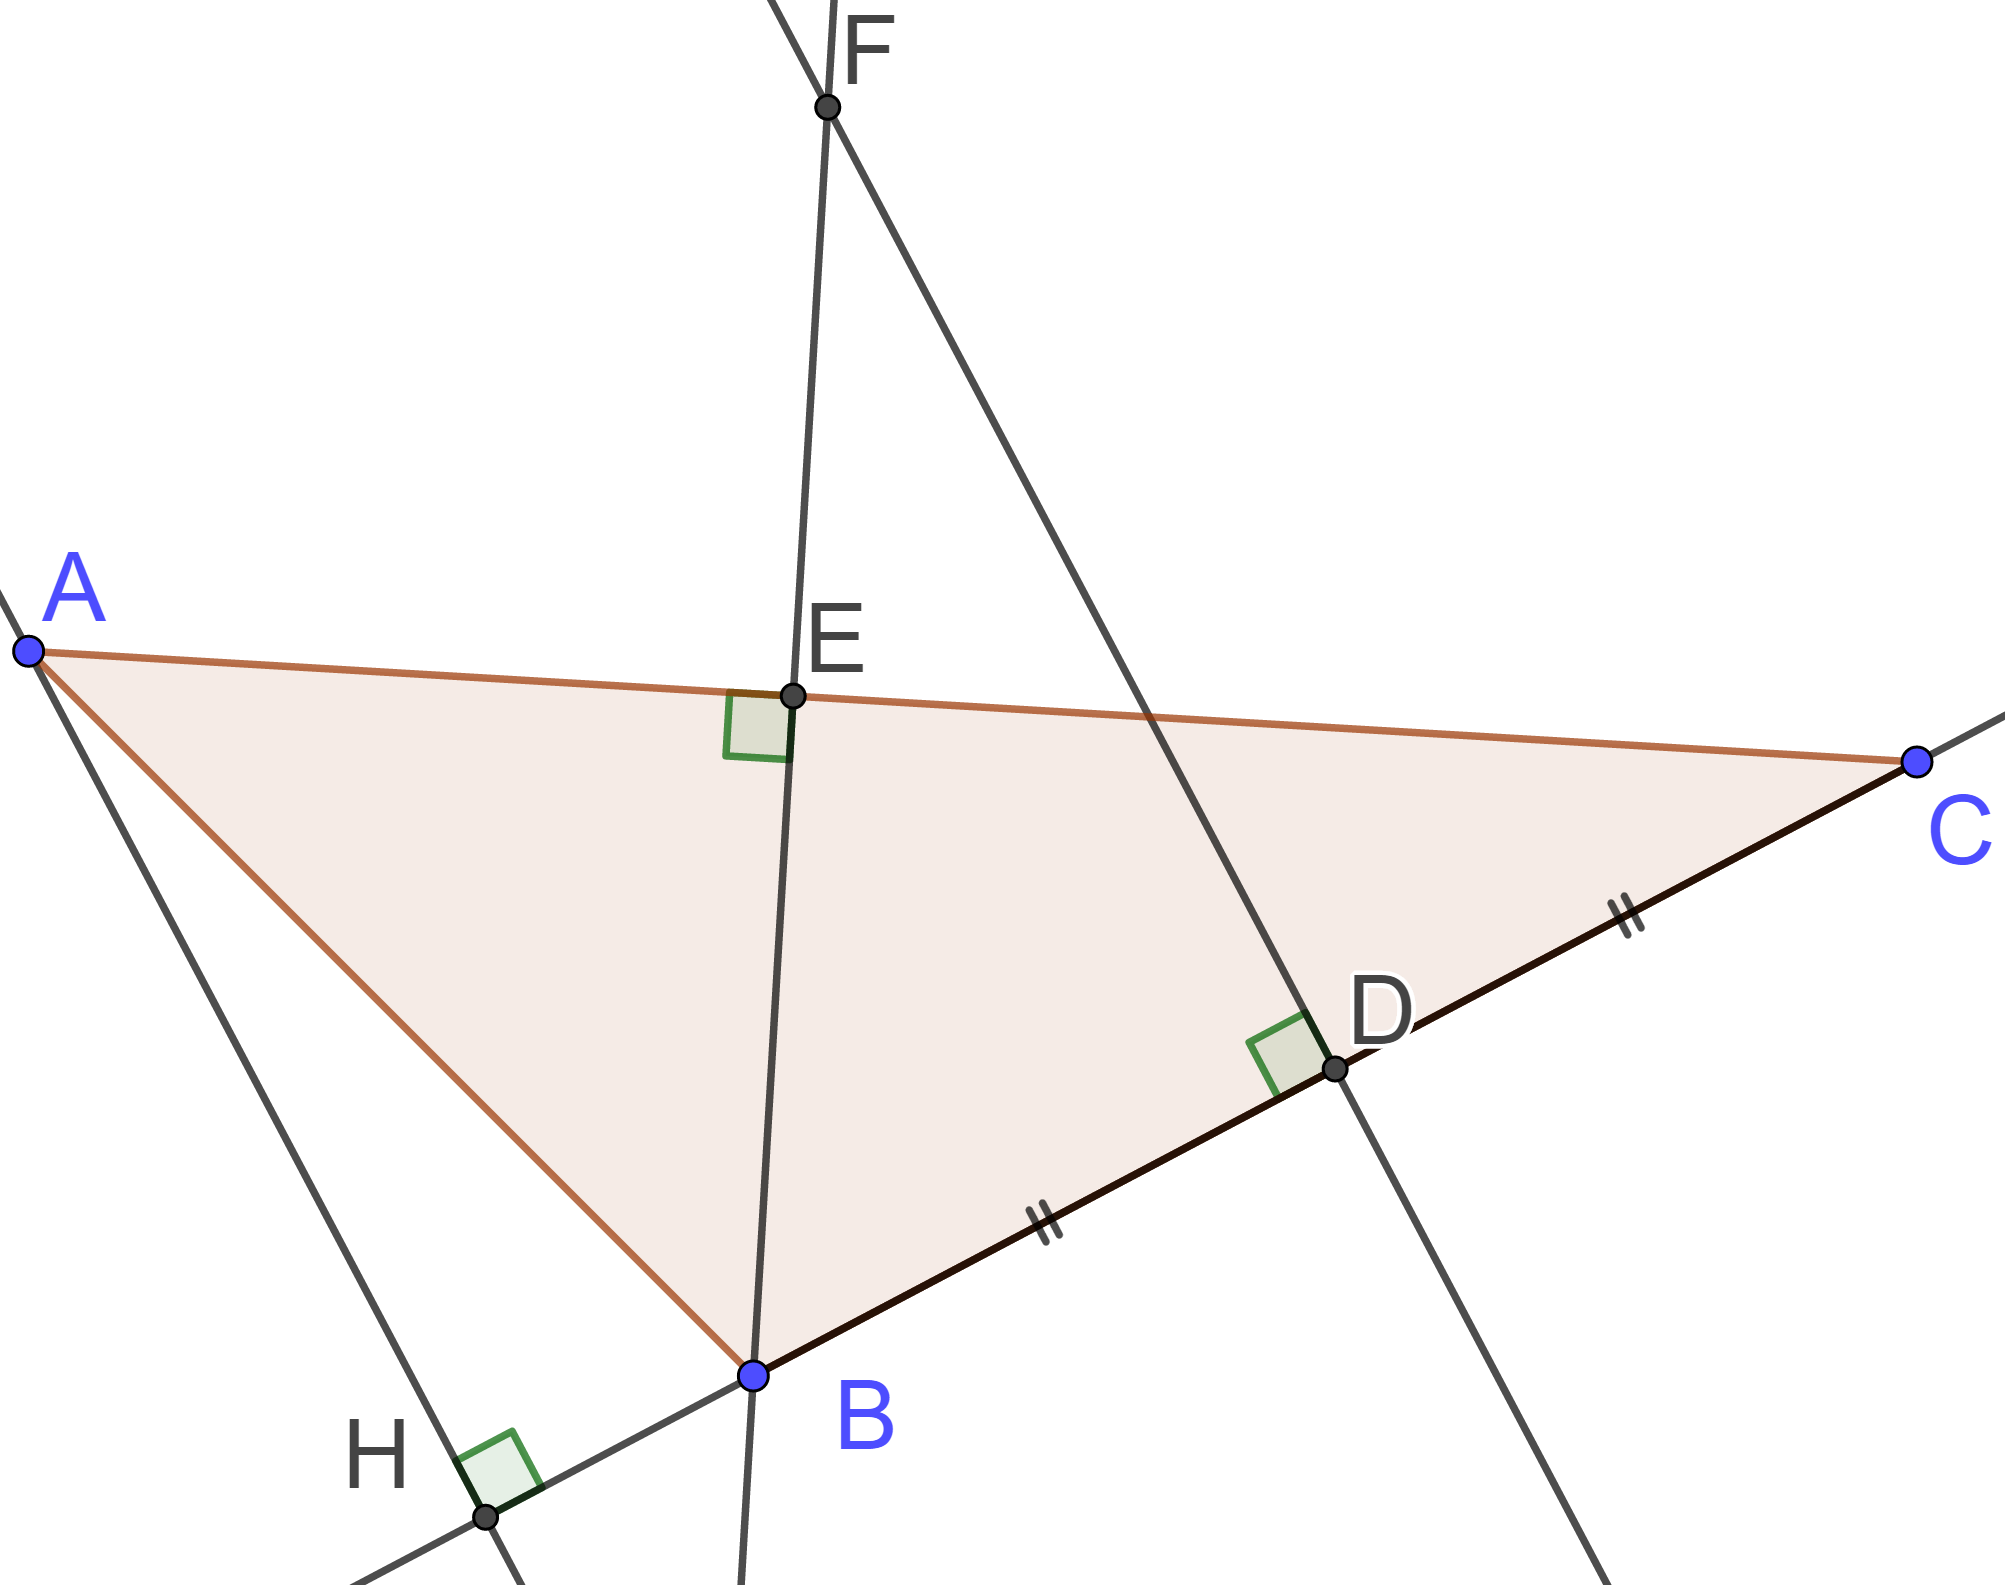
\includegraphics[scale=0.15]{droites}
		\end{center}
	\end{multicols}
\end{myexs}